\chapter{Conclusion \label{chapter4_conclusion}}


\section{Measurements of the Properties of the Higgs Boson}

The collaborations \CMS and \ATLAS combined their measurements after Run 1 in order to measure the Higgs mass and
the coupling to fermions with higher precision.

The combination of the Higgs mass was measured in the $\PH \rightarrow \PZ \PZ \rightarrow 4\Plepton$ and
$\PH \rightarrow \Pgamma \Pgamma$ channel. A likelihood fit was performed in order to extract the best fit result for
$m_H$ from data. Figure~\ref{figure_higgs_mass} shows the likelihood parabola, where the minimum depicts the best fit value for $m_H$. Furthermore
one can directly extract the $1\sigma$ ($2\sigma$) uncertainty from this plot by looking at the value for $m_H$ for $-2\mathrm{ln} \Lambda(m_H)=1 \,(4)$.
The best fit value for the Higgs mass was determined to be:
$m_H=125.09 \pm 0.21 \text{(stat.)} \pm 0.11 \text{(syst.)}$ GeV.

\begin{figure}[h]
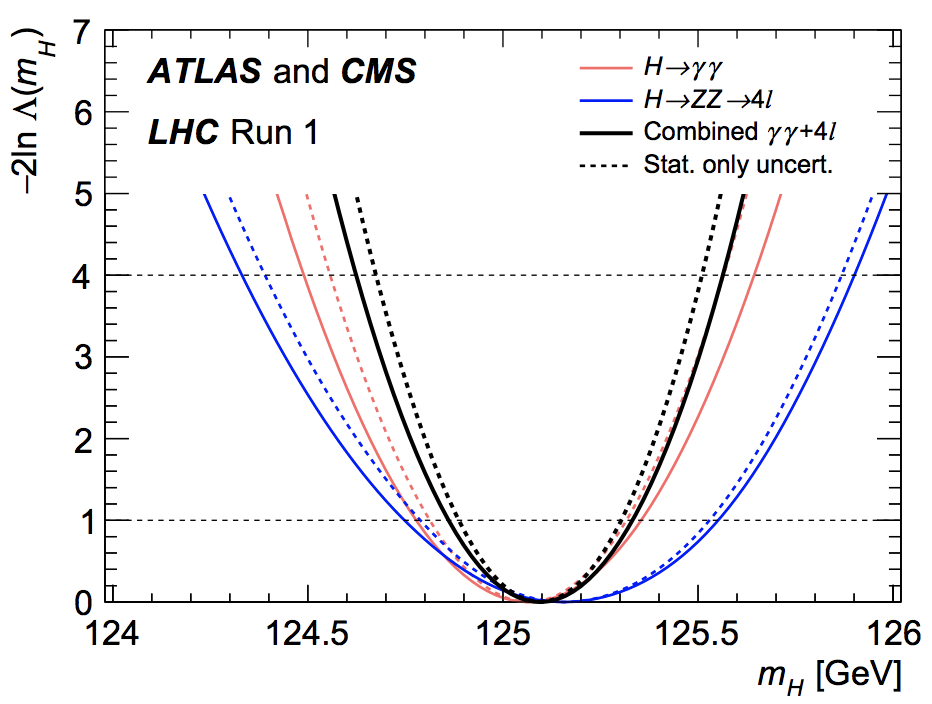
\includegraphics[width=0.75\textwidth]{../plots/higgsmass}
\caption[Higgs boson mass.]{Combined likelihood fit of the Higgs boson mass by \ATLAS and \CMS~\cite{HiggsMass}.}
\label{figure_higgs_mass}
\end{figure}

As aforementioned the Higgs coupling was measured in a combined measurement. The coupling strength of the Higgs boson was predicted
to be proportional to the mass of the fermions or vector bosons. It is shown in figure~\ref{figure_higgs_coupling}, that this predictions holds
within the uncertainties of the data points. A deviation in data from this fit would already be a clear hint to something new. Therefore it is necessary to study
all the SM Higgs boson decays with a very high precision.

\begin{figure}[h]
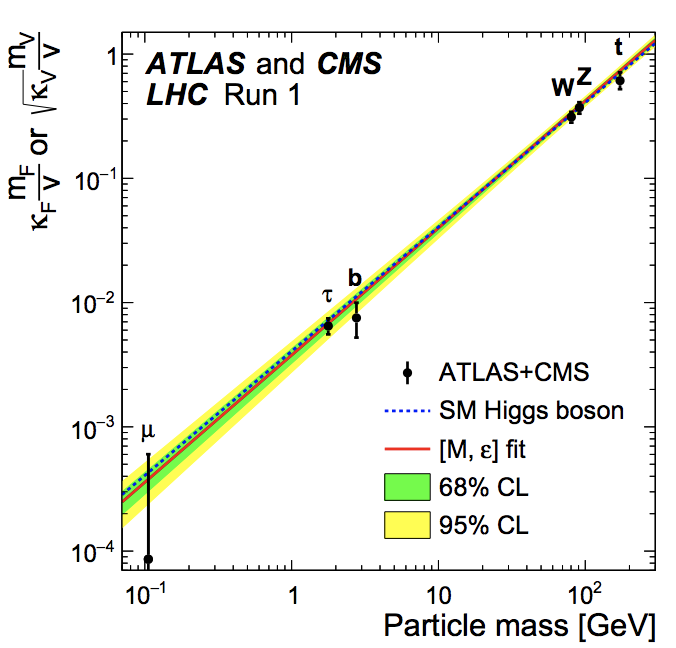
\includegraphics[width=0.75\textwidth]{../plots/higgscoupling_masses}
\caption[Higgs boson coupling.]{Higgs coupling to fermions or vector bosons as a function of the particle massesn by \ATLAS and \CMS~\cite{HiggsMass}.}
\label{figure_higgs_coupling}
\end{figure}

By measuring the SM Higgs decaying into a pair of photons and a pair of tau leptons it is directly clear that the measured Higgs boson is a spin-0 particle and
electrically neutral. Unfortunately the amount of data is still too low to measure the CP eigenvalue of the Higgs boson. The SM Higgs is predicted to have a
CP eigenvalue of +1. A deviation of this value in a measurement would directly point to physics beyond the SM (BSM).

\section{Exciting Times Ahead...}

With the observation of a new scalar boson in July 2012 a milestone in particle physics was set. Now it is essential to measure all the properties
of the Higgs boson with very high precision. Furthermore the Higgs boson can be used as a probe for new physics. Searches for dark matter produced in
association with a Higgs boson are already ongoing. It is still not clear if there is only one Higgs boson or even more. Many BSM theories (like supersymmetry) require two Higgs doublets, which
predict in total 5 Higgs bosons. Obviously these discoveries are only possible with upgrades in the experiments \CMS and \ATLAS and the accelerator \LHC.

At \LHC there is a future plan until 2035 to upgrade the experiment after Run 3 to a high luminosity machine (HL-LHC). The timetable is shown in figure~\ref{figure_hllhc}.

\begin{figure}[h]
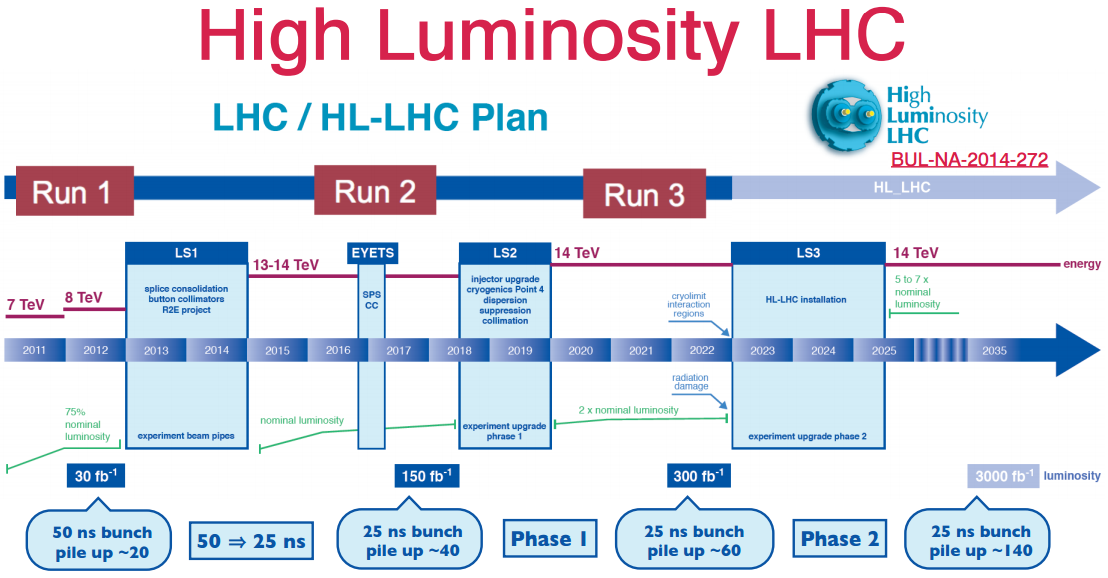
\includegraphics[width=0.75\textwidth]{../plots/hllhc.png}
\caption[HL-LHC]{Future plan of \LHC. A high luminosity upgrade is planned after Run3 until 2035~\cite{HL-LHC}.}
\label{figure_hllhc}
\end{figure}

This upgrade will have some consequences. The main consequence is an increase in pile-up events, which makes data reconstructing even harder than before.
Also an increased amount of data is very challenging for the trigger systems and storage systems.

A new experiment is currently planned in Japan, the so-called International Linear Collider (ILC). Its main purpose is to measure
the mass, the interaction strengths and the CP properties of the Higgs boson with a very high precision. An accelerator of this kind is often referred to as
a Higgs-factory.

All of these developments in Higgs physics will keep the future very interesting. New exciting results will definitely pop up in the near future.
